\chapter{KẾT QUẢ HIỆN TẠI ĐẠT ĐƯỢC}
\section{Kết quả đánh giá trên tập Test}
FVC và Confidence tìm được khi sử dụng mô hình Efficient Net được lưu vào một file .csv như hình \ref{fig:res1} tạm gọi là tập sub để đánh giá tổng hợp.\par
\begin{figure}[ht!]
\centerline{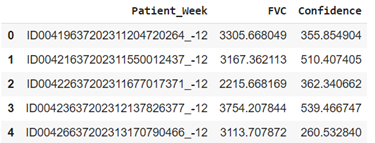
\includegraphics[scale=1.2]{images/res1.png}}
\caption{FVC và Confidence dự đoán được từ mô hình với 5 bệnh nhân ở tuần -12}
\label{fig:res1}
\end{figure} 
Các dữ liệu của bệnh nhân đưa vào mô hình Quantile Regression để dự đoán ra FVC(QR).Hình \ref{fig:res2} là kết quả dự đoán qua mô hình Quantile Regression của bệnh nhân có ID là “ID00419637202311204720264”.\par
\begin{figure}[ht!]
\centerline{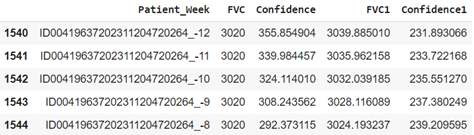
\includegraphics[scale=1.1]{images/res2.png}}
\caption{FVC dự đoán của mô hình với bệnh nhân “ID00419637202311204720264” với 5 tuần từ tuần -12 tới tuần -8, FVC1 và Confidence 1 là kết quả dự đoán của mô hình}
\label{fig:res2}
\end{figure}
Hai kết quả trên được tính toán theo công thức đã nêu $FVC= FVC(EF)*0.45+ FVC(QR)*0.55$ để tính toán ra FVC cuối cùng:\par
\begin{figure}[ht!]
\centerline{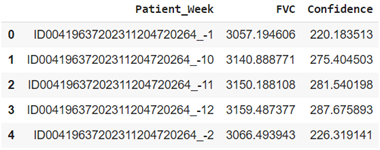
\includegraphics[scale=1.0]{images/res3.png}}
\caption{FVC và Confidence dự đoán cuối cùng từ 2 mô hình ở một số tuần của bệnh nhân “ID00419637202311204720264”}
\label{fig:res3}
\end{figure}

Thực hiện dự đoán trên 5 bệnh nhân với mỗi bệnh nhân gồm 9 giá trị FVC ở các tuần khác nhau ở tập kiểm tra, kết quả của mô hình cho thấy trung bình mỗi bệnh nhân cho thấy có khoảng từ 0 đến 2 giá trị FVC của bệnh nhân bị tính sai trong khoảng từ Confidence. Như vậy, khả năng dự đoán chính xác của mô hình vào khoảng 76.9231$\%$. Các giá trị dự đoán sai khỏi khoảng Confidence cũng không quá cao, không vượt quá 300.\par
Ngoài ra độ lệch trung bình giữa FVC đúng so với FVC chính xác (lượng tử là 0.5) là 126.8966 
Mô hình có tỉ lệ dự đoán chính xác khác cao, tuy nhiên vẫn còn hạn chế. Việc vẫn còn hạn chế nằm ở tập các giá FVC của các bệnh nhân chưa đủ nhiều, việc xây dựng mô hình hồi quy tuyến tính còn hạn chế và do hạn chế ở RAM tính toán nên việc phải resize ảnh chụp CT từ 512 x 512 về còn 64 x 64 khiến mô hình dự đoán thiếu chính xác.
